% Created 2019-07-11 Thu 12:01
% Intended LaTeX compiler: pdflatex
\documentclass[11pt]{article}
\usepackage[utf8]{inputenc}
\usepackage[T1]{fontenc}
\usepackage{graphicx}
\usepackage{grffile}
\usepackage{longtable}
\usepackage{wrapfig}
\usepackage{rotating}
\usepackage[normalem]{ulem}
\usepackage{amsmath}
\usepackage{textcomp}
\usepackage{amssymb}
\usepackage{capt-of}
\usepackage{hyperref}
\usepackage{listings}
\usepackage[left=1in,top=1in,right=1in,bottom=1in]{geometry}
\usepackage{palatino}
\usepackage{fancyhdr}
\usepackage{sectsty}
\usepackage{engord}
\usepackage{cite}
\usepackage{graphicx}
\usepackage{setspace}
\usepackage[compact]{titlesec}
\usepackage[center]{caption}
\usepackage{multirow}
\usepackage{ifthen}
\usepackage{longtable}
\usepackage{color}
\usepackage{amsmath}
\usepackage{listings}
\usepackage{pdfpages}
\usepackage{nomencl}	% For glossary
\usepackage{pdflscape}	% For landscape pictures and environment
\usepackage{verbatim} 	% For multiline comment environments
\usepackage[table]{xcolor}
\author{eo shiru}
\date{\today}
\title{SVS - Tutorials}
\hypersetup{
 pdfauthor={eo shiru},
 pdftitle={SVS - Tutorials},
 pdfkeywords={},
 pdfsubject={},
 pdfcreator={Emacs 26.2 (Org mode 9.1.9)}, 
 pdflang={English}}
\begin{document}

\maketitle
\tableofcontents

\section{Nmap, Attack Targets, HTTP Headers \& Statusses}
\label{sec:org4d0b49b}
\begin{center}
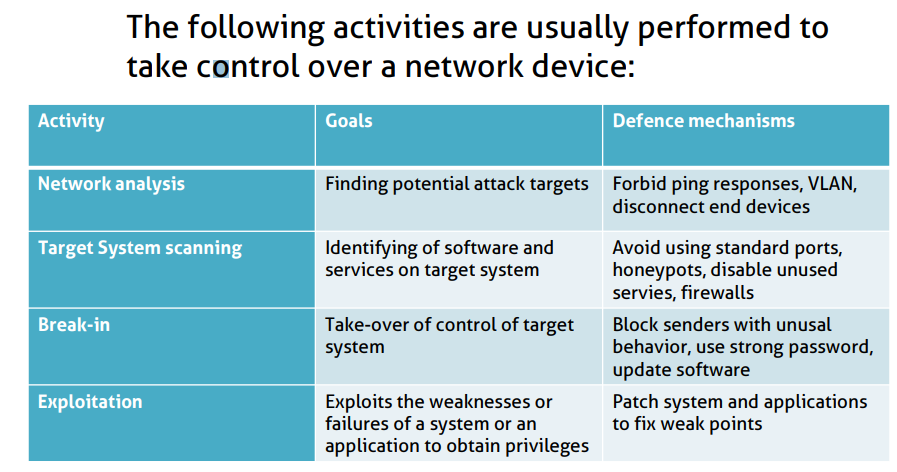
\includegraphics[width=.9\linewidth]{./F7.png}
\end{center}
\begin{itemize}
\item tools for 
\begin{itemize}
\item target system scanning \(\rightarrow\) nmap
\begin{itemize}
\item scan a single IP \(\rightarrow\) \texttt{nmap 192.168.1.1}
\item scan specific IPs \(\rightarrow\) \texttt{nmap 192.168.1.1 192.168.2.1}
\item scan a range \(\rightarrow\) \texttt{nmap 192.168.1.1-254}
\item \texttt{-sV -{}-version-all} for service detection
\item flag \texttt{-A} or \texttt{-O} for OS detection
\item reverse DNS: \texttt{nmap -v -sn 192.168.0.0/24 \# sucht alle rechner mit der IP 192.168.0.*}
\item services on host: \texttt{nmap -T4 -O -F tan.informatik.tu-chemnitz.de}
\end{itemize}
\item network analysis \(\rightarrow\) Cain \& Abel, Wireshark
\item break-in \(\rightarrow\) Hydra
\end{itemize}
\item Example IT entities which can become a target for an attack: Users, Applications, Operating Systems, End devices, Networks
\end{itemize}
\begin{center}
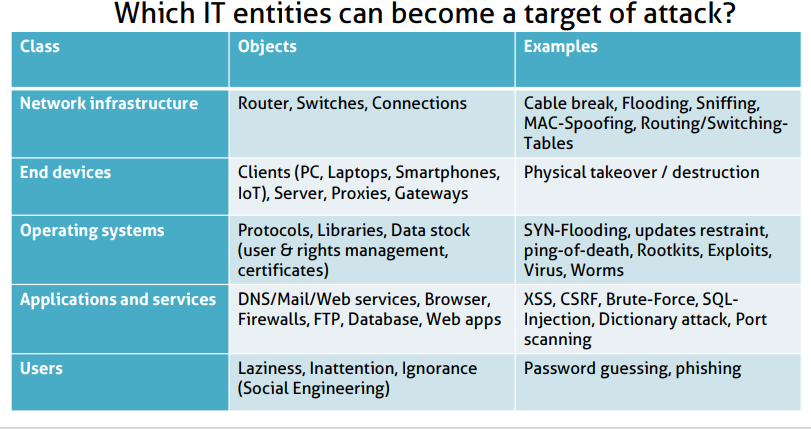
\includegraphics[width=.9\linewidth]{./F3.png}
\end{center}
\begin{itemize}
\item "HTTP/1.0, includes the specification for a Basic Access Authentication scheme. This scheme is not considered to be a secure method of user authentication (unless used in conjunction with some external secure system such as SSL), as the user name and password are passed over the network as cleartext."
\begin{itemize}
\item headers: \texttt{WWW-Authenticate: <type> realm=<realm>} response header defines the authentication method that should be used to gain access to a resource and \texttt{Authorization: <type> <credentials>} from request (user) to authenticate
\begin{itemize}
\item Bei dem WWW-Authenticate: Basic Verfahren, werden Benutzername und Passwort unverschlüsselt an den Server übertragen. Dabei werden die Zugangsdaten in dem HTTP Header Authorization in der folgenden Form übertragen zB \texttt{Authorization: Basic base64\_encode(Benutzername:Passwort)} d.h. Benutzername und Passwort wird mit einem Doppelpunkt verbunden und mit Base64 codiert (nicht verschlüsselt!).
\end{itemize}
\end{itemize}
\end{itemize}
Codierung ist nur eine andere Darstellung der Quelldaten und kann mit Kenntnis des Verfahren ohne Probleme codiert und decodiert werden

\begin{itemize}
\item The \texttt{Host} request header (\texttt{Host: <host>:<port>}) specifies the domain name of the server (for virtual hosting), and (optionally) the TCP port number on which the server is listening. If no port is given, the default port for the service requested (e.g., "80" for an HTTP URL) is implied (eg \texttt{Host: developer.cdn.mozilla.net})
\item The \texttt{Accept} request HTTP header advertises which content types, expressed as MIME types, the client is able to understand. Using content negotiation, the server then selects one of the proposals, uses it and informs the client of its choice with the \texttt{Content-Type} response header.
\end{itemize}

1xx (Informational): The request was received, continuing process\\
2xx (Successful): The request was successfully received, understood and accepted\\
3xx (Redirection): Further action needs to be taken in order to complete the request\\
4xx (Client Error): The request contains bad syntax or cannot be fulfilled\\
5xx (Server Error): The server failed to fulfill an apparently valid request\\
\section{SQL Injection}
\label{sec:orgca66d95}
\begin{itemize}
\item What is Session Hijacking?
\begin{itemize}
\item The Session Hijacking attack consists of the exploitation of the web session control mechanism, which is normally managed for a session token.
\end{itemize}
\item How do you get a Session-Token?
\begin{itemize}
\item Predictable Session Token
\item Session Sniffing
\item Client-side attacks (XSS)
\end{itemize}
\item set "session" cookie via JS: \texttt{document.cookie="session=John";}
\item What is SQL-Injection?
\begin{itemize}
\item A SQL injection attack consists of insertion or "injection" of a SQL query via the input data from the client to the application
\end{itemize}
\item What can be done with SQL Injection?
\begin{itemize}
\item …read sensitive data from the database, modify database data (Insert/Update/Delete), execute administration operations on the database (such as shutdown the DBMS), recover the content of a given file present on the DBMS file system and in some cases issue commands to the operating system
\end{itemize}
\item a SQL query can be injected via form data, url parameters, cookies
\item SQL injection example (not sanitized form fields):
\begin{itemize}
\item one input field 'name': enter Max you get: \texttt{SELECT * FROM personen WHERE name = 'Max'}, enter Max' OR name LIKE '\% and you get \texttt{SELECT * FROM personen WHERE name = 'Max' OR name LIKE '\%'} which gives you all persons
\item two inputs name and password: enter user1 in the name input field and pass1' OR username LIKE '\% in the password field to get all users with their respective passphrases
\end{itemize}
\item SQL-Injection Protection:
\begin{itemize}
\item Filter or mask special chars
\item Check input values for properties
\item Black-/Whitelisting of parameters
\item Seperation of Data and SQL-Queries
\item Fine Distinction of user rights
\item Disable unused DB functionalites
\item Apply Web Application Firewalls
\end{itemize}
\end{itemize}
\section{Cross-Site-Scripting (XSS)}
\label{sec:org2f11741}
\begin{center}
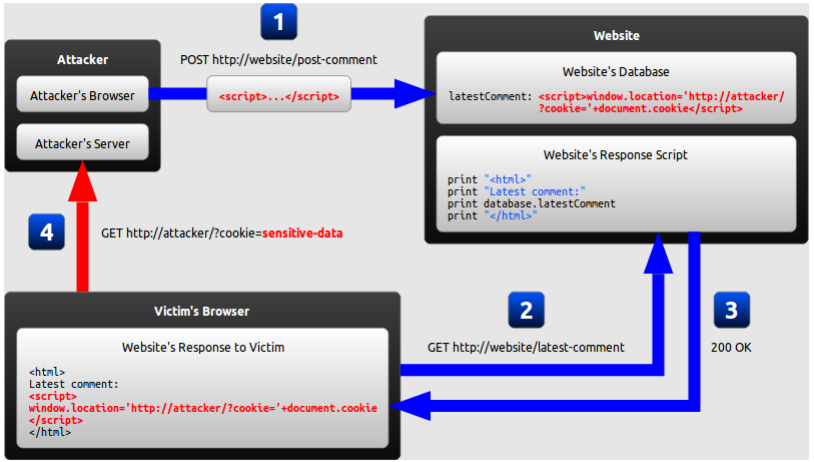
\includegraphics[width=.9\linewidth]{./F10.png}
\end{center}
\begin{center}
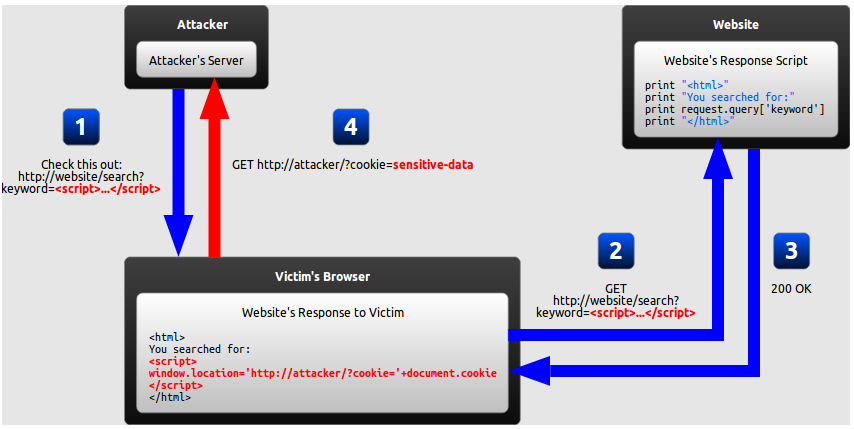
\includegraphics[width=.9\linewidth]{./F11.png}
\end{center}
\begin{center}
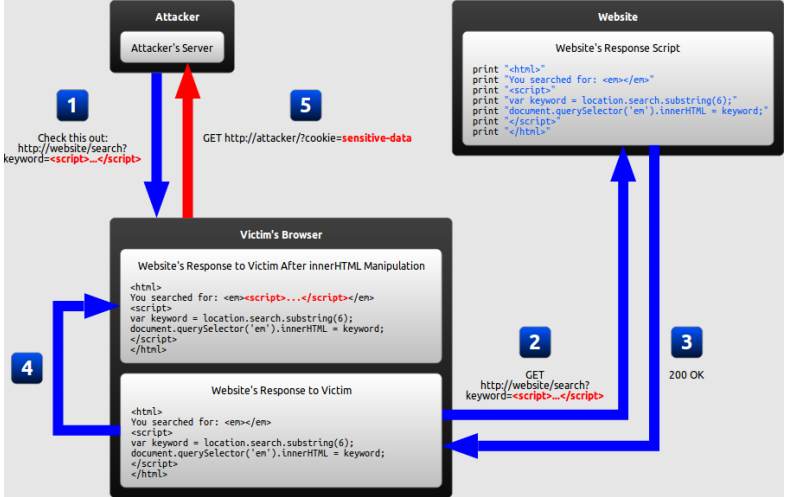
\includegraphics[width=.9\linewidth]{./F12.png}
\end{center}
\begin{itemize}
\item What is Cross-Site Scripting (XSS)?
\begin{itemize}
\item Cross-Site Scripting attacks are a type of injection problem, in which malicious scripts are injected into the otherwise benign and trusted web sites
\end{itemize}
\item What is achievable with XSS?
\begin{itemize}
\item Spy out data (incl. Cookie / Session variables)
\item Altering website
\item Phishing
\end{itemize}
\item Which defense methods against XSS do you
\end{itemize}
know?
\begin{itemize}
\item Validate user inputs
\item Encode output
\item Use HttpOnly flag for cookies
\item Deactivate JavaScript in the browser
\item Web Application Firewalls
\end{itemize}
\begin{itemize}
\item Example input form:
\begin{itemize}
\item insert <script>JSCODE</script> to do whatever you want
\end{itemize}
\item What is the difference between stored, reflected and DOM-based XSS attacks?
\begin{itemize}
\item Stored XSS Attacks = Malicious code stored on server side – forums, guestbooks etc.
\item Reflected XSS Attacks = Malicious code delivered to the client, but not stored on the server side
\item DOM-based Attacks = Malfunction of normal code behavior via manipulated parameters
\end{itemize}
\item Example XSS Input:
\end{itemize}
\lstset{breaklines=true,language=javascript,label= ,caption= ,captionpos=b,numbers=none}
\begin{lstlisting}
<script type="text/javascript">
function cookie_lesen() {
  document.cookie="username=John Doe;" + document.cookie;
  alert("Deine Cookies:\n\n" + document.cookie);
  // hier könnte man natürlich die Kekse an ein fremdes System schicken...
}
</script>

<a onclick="cookie_lesen()" href="#">cookies</a>
\end{lstlisting}
\lstset{breaklines=true,language=javascript,label= ,caption= ,captionpos=b,numbers=none}
\begin{lstlisting}
<script type="text/javascript">
function farbe_aendern() {
  var h1 = document.getElementsByTagName("h1")[0];
  h1.setAttribute("style", "color:red;");
}
function links_aendern() {
  var links = document.getElementsByTagName("a");
  var i;
  for (i = 0; i<links.length;i++) {
    links[i].href = "http://google.de/";
  }
}
farbe_aendern();
links_aendern();
</script>
\end{lstlisting}
\begin{itemize}
\item Logout via JS:
\begin{itemize}
\item invalidate cookies \(\rightarrow\) document.cookie += "; expires=Thu, 01 Jan 1970 00:00:01 GMT;"
\item location.reload()
\end{itemize}
\item The same-origin policy is a critical security mechanism that restricts how a document or script loaded from one origin can interact with a resource from another origin (origin = protocol + port + host). It helps isolate potentially malicious documents, reducing possible attack vectors.
\begin{itemize}
\item the first iFrame has same domain and port, the second iFrame refers to another domain and the access is therefore restricted by the same-origin-policy
\end{itemize}
\end{itemize}
\lstset{breaklines=true,language=javascript,label= ,caption= ,captionpos=b,numbers=none}
\begin{lstlisting}
var h1_first_frame = window.frames[0].document.getElementsByTagName("h1")[0].innerHTML;
 window.frames[1] // undefined
\end{lstlisting}
\begin{itemize}
\item Cross-Site-Request-Forgery (CSRF) = is an attack that forces an end user to execute unwanted actions on a web application in which they're currently authenticated. CSRF attacks specifically target state-changing requests, not theft of data, since the attacker has no way to see the response to the forged request. With a little help of social engineering (such as sending a link via email or chat), an attacker may trick the users of a web application into executing actions of the attacker's choosing. If the victim is a normal user, a successful CSRF attack can force the user to perform state changing requests like transferring funds, changing their email address, and so forth. If the victim is an administrative account, CSRF can compromise the entire web application.\\
\end{itemize}
For example:
\lstset{breaklines=true,language=javascript,label= ,caption= ,captionpos=b,numbers=none}
\begin{lstlisting}
<img src="http://meine-bank.example.com/?logout=1">
// or
<img src="http://meine-bank.example.com/transfer-money?from=123&to=321&amount=1024">
// or
<href="https://www-user.tu-chemnitz.de/~cole/svs/03/session.php?logout=1">Schaut mal, tolle Sache hier</a>
\end{lstlisting}

\section{Hashing, Keys and Encryption}
\label{sec:org48750db}
\begin{itemize}
\item Where to use one-way hash functions?
\begin{itemize}
\item Transmit error detection
\item Fast data access
\item Identification/Comparison of secrets
\end{itemize}
\item Criteria of a good one-way hash function:
\begin{itemize}
\item Pre-image resistance, irreversibility
\item Second pre-image resistance, collision resistance
\item Efficient calculable
\item High dispersion ↔ order preservation* SVS-Tutorial\(_{\text{06.pdf}}\)
\end{itemize}
\item Example: Encode message "VSR" using the ASCII table and hash function \(f(s) = (\sum_{i=1}^{\text{length}(s)} s_i) % 7\)
\begin{itemize}
\item f("VSR") = (86 + 83 + 82) mod 7 = 251 mod 7 = 6
\end{itemize}
\item Example: Create MD5 hash of "VSR": \texttt{echo -n "VSR" | md5sum} for eg sha265 use \texttt{sha265sum} or via gpg: \texttt{echo -n "VSR" | gpg -{}-print-md md5}
\item Caesar Cipher
\begin{itemize}
\item Advantages
\begin{itemize}
\item Fast Algorithms
\item Easy Hardware implemenation
\end{itemize}
\item Disadvantages
\begin{itemize}
\item requires secure channel
\item requires key administration
\end{itemize}
\item Security Risks
\begin{itemize}
\item Frequency Analysis
\item Brute-Force
\item concealment of approach not key
\end{itemize}
\end{itemize}
\item Example: Encrypt message M = "DE" using RSA encryption with public key (\(e=7\), \(N=77\))
\begin{enumerate}
\item Turn M into \textbf{one} number m which is smaller than N: convert to numbers D \(\rightarrow\) 4, E \(\rightarrow\) 5 (positions in alphabet) \(\rightarrow\) \(4+5 =9\)
\item Compute ciphertext c: \(c = m^e \mod N\)
\item \$c = 9\(^{\text{7}}\) \mod 77 = 37
\item Send c to partner
\item Recover m from c using via private key (\(d=43\), \(N=77\)): \(m=c^d \mod N\)
\item \(m = 37^43 \mod 77 = 9\)
\end{enumerate}
\item Using gpg
\begin{itemize}
\item \texttt{gpg -{}-full-generate-key} to generate key-pair (RSA)
\item send public key to recipient 
\begin{itemize}
\item via a file: \texttt{gpg -{}-armor -{}-output mypubkey.gpg -{}-export your.name@yourdomain.com}
\item via public key server: \texttt{gpg -{}-list-secret-keys} to find out public key id which stands next to "sec" and then export via \texttt{gpg -{}-send-keys KEYID} and note the GPG server
\end{itemize}
\item encrypting a file: \texttt{gpg -{}-output myfile.txt.gpg -{}-encrypt -{}-recipient your.friend@yourfriendsdomain.com  myfile.txt}
\item decrypting a file: \texttt{gpg -{}-output myfile.txt -{}-decrypt myfile.txt.gpg}
\end{itemize}
\item signing a message so that the recipient can verify that it is indeed by the sender:
\begin{itemize}
\item private key = (d=27, N=55); public key = (e=3, N=55); message m = "DE" \(\rightarrow\) 9
\item \(s= m^d \mod N\) = 9\(^{\text{27}}\) \mod 55 = 4\$
\item send message (9) and signature (4) to recipient
\item recipient verifies the message via \(m = s^e \mod N\)
\item \(m = 4^3 \mod 55 = 9\) \(\rightarrow\) correct!
\end{itemize}
\item Alice sends \(m\) through the public channel and \(h(m)\) through the *integrity\$ channel where \(h\) is a cryptgraphic hash function
\item \textbf{authenticity} via verifying keys
\begin{itemize}
\item symmetric: secret key \(K\) is generated and sent to Alice \& Bob, Alice sends (m, MAC(m, K)) through public channel and Bob verifies via \(\text{VERIF}(m,K)\); MAC is a hash function parameterized by K
\item asymmetric: a key pair (\(K_s\), \(K_p\)) is generate dby Alice and she sends the public key \(K_p\) to Bob via public channel and she sends \((m, \text{SIGN}(m, K_s))\) through public channel and Bob verifies via \(\text{VERIF}(m, K_p)\)
\end{itemize}
\item \textbf{confidentiality} via permutation (encryption \& decryption)
\begin{itemize}
\item symmetric: secret K is generated and sent to Alice \& Bob, Alice sends \(c=E(m,K)\) and Bob decrypts via \(m=D(c,K)\)
\item asymmetric: key pair (K\(_{\text{s}}\), K\(_{\text{p}}\)) is generated by Bob and he sends public key K\(_{\text{p}}\) to Alice who then sends \(c=E(m,K_p)\) to Bob who decrypts this via \(m=D(C, K_s)\)
\end{itemize}
\item X.509 is a standard defining the format of public key certificates, X.509 certificates are used in many Internet protocols, including TSL/SSL which is the basis for HTTPS
\begin{itemize}
\item contains a public key, an identity (hostname, organization, individual) and is either signed by a certificate authority or self-signed
\end{itemize}
\item In public key infrastructure (PKI) systems, a certificate signing request (also CSR or certification request) is a message sent from an applicant to a certificate authority in order to apply for a digital identity certificate. It usually contains the public key for which the certificate should be issued, identifying information (such as a domain name) and integrity protection (e.g., a digital signature)
\item create self signed cert via openssl: \texttt{openssl req -new -newkey rsa:4096 -x509 -sha256 -days 365 -nodes -out MyCertificate.crt -keyout MyKey.key}
\end{itemize}

\textbf{Symmetrische Verfahren}
\begin{itemize}
\item Integritätssicherstellung mit Hash. Wichtiges Kriterium der Hash's: Kollisionsfreiheit.
\item Authentizität: Woher weiß Bob, dass Nachricht von Alice kommt? Niemand kennt privaten Schlüssel.
\end{itemize}

\textbf{Asymmetrische Verfahren}
\begin{itemize}
\item Kein Austausch von Schlüsseln; jeder generiert sich ein Schlüsselpaar. Jeder Kommunikationspartner hat die öffentlichen Schlüssel von den Anderen. Wenn Alice an Bob eine Nachricht schreibt, verwendet sie den Public-Key zum Verschlüsseln und Bob verwendet seinen Private-key zum entschlüsseln.
\end{itemize}

\textbf{Vertraulichkeit} = Private-Key ist nur dem Sender bekannt.

\textbf{Integrität} = Man kann blind versuchen die Nachricht zu manipulieren, z.B. Nachrichtenteil anhängen (der zweite Teil wird dann einfach wieder mit dem Public-Key verschlüsselt). Darum sollte man die Nachricht vor dem Versenden mit einem Hash versehen. Hashwert wird mitverschlüsselt.

\textbf{Authentizität} = Bob bekommt Nachricht mit Hash (von Alice). Woher weiß er, wer die Nachricht versendet hat?
\begin{itemize}
\item Signatur wird erstellt mit Private-Key von Alice über Hashwert der Nachricht.
\item Bob kann Signatur mit Public-Key von Alice entschlüsseln und Authentizität feststellen.
\end{itemize}

\section{SSL/TLS (+ HTTP, SSH)}
\label{sec:orgbd2aabf}
\begin{center}
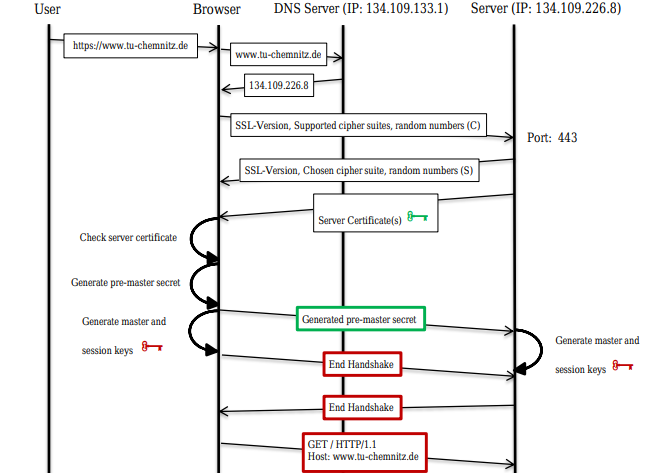
\includegraphics[width=.9\linewidth]{./F32.png}
\end{center}
\begin{itemize}
\item Hostname wird an DNS Server übertragen
\item IP-Adresse kommt zurück
\item Port: 443
\item Server sendet Zufallszahl Random\(_{\text{S}}\), gewählte Cipher Suite, SSL-Version
\item Überprüfung des Zertifikats
\begin{itemize}
\item Anhand des Zertifikatspeichers des Browsers, bspw. bei selbst signierten Zertifikaten
\item Signatur von Zertifikat, wird geprüft, ob öffentlicher Schlüssel im Browser bekannt ist
\end{itemize}
\item Auf Basis von den 3 Zufallszahlen wird auf Client-Seite auch Primär- und Sizungs-Schlüssel generiert
\item Server-End-Handshake, als Antwort auf Client-End-Handshake
\item GET / HTTP/1.1, Host: www.tu-chemnitz.de
\end{itemize}
\begin{itemize}
\item Which goals does SSL/TLS have?
\begin{itemize}
\item confidentiality
\item authenticity
\item integrity
\end{itemize}
\item Which risks exist despite of usage of SSL/TLS?
\begin{itemize}
\item out-of-scope
\end{itemize}
\item How does the server decide which certificate should be shown if several virtual hosts exist?
\begin{itemize}
\item Server Name Indication (SNI)
\item Wildcard Certificates
\item Multidomain-Certificates
\end{itemize}
\item HTTP Digest Authentication
\begin{itemize}
\item Pro:
\begin{itemize}
\item prevent phishing
\item no password storage at apps
\item prevents chosen-plaintext attacks
\item prevents replay attacks
\end{itemize}
\item Con:
\begin{itemize}
\item many security options are optional
\item man-in-the-middle attack
\item prevents strong hash algorithms
\end{itemize}
\item What would a client send as a response to the following server message, if his username would be „Max“ and his password - „Secure123“?
\begin{itemize}
\item Request (Client):
\lstset{breaklines=true,language=bash,label= ,caption= ,captionpos=b,numbers=none}
\begin{lstlisting}
GET /index.html HTTP/1.1
Host: localhost
\end{lstlisting}
\item Response (Server):
\lstset{breaklines=true,language=bash,label= ,caption= ,captionpos=b,numbers=none}
\begin{lstlisting}
HTTP/1.0 401 Unauthorized
WWW-Authenticate: Digest realm="Secured Area",
nonce="aer95b7fg2dd2hhe8b11d0f6f7afb0c14v"
Content-Length: 0
\end{lstlisting}
\item Client:
\begin{itemize}
\item HA1 = MD5(username:realm:password)
\item HA2 = MD5(method:digestURI)
\item response = MD5(HA1:nonce:HA2)
\end{itemize}
\end{itemize}
\end{itemize}
\item SSH Public Key Authentication
\begin{itemize}
\item create key: \texttt{ssh-keygen -t rsa -C "my\_email@example.com"}
\item transfer to server: \texttt{cat \textasciitilde{}/.ssh/id\_rsa.pub | ssh username@server.address.com 'cat >> \textasciitilde{}/.ssh/authorized\_keys'} (ssh agent needs to be running for this)
\begin{itemize}
\item alternative: \texttt{ssh-copy-id –i .ssh/id\_rsa.pub \{user\}@\{server\}}
\end{itemize}
\item test authentication via \texttt{ssh \{user\}@\{server\}}
\end{itemize}
\end{itemize}
\section{Kerberos}
\label{sec:org434d97a}
\subsubsection{Kerberos Procedure}
\label{sec:org62fe5e2}
\textbf{Description}
\begin{itemize}
\item The client authenticates itself to the Server (AS) which forwards the username to a key distribution center (KDC). The KDC issues a ticket-granting ticket (TGT), which is time stamped and encrypts it using the ticket-granting service's (TGS) secret key and returns the encrypted result to the user's workstation. This is done infrequently, typically at user logon; the TGT expires at some point although it may be transparently renewed by the user's session manager while they are logged in.
\item When the client needs to communicate with another node ("principal" in Kerberos parlance) to some service on that node the client sends the TGT to the TGS, which usually shares the same host as the KDC. Service must be registered at TGT with a Service Principal Name (SPN). The client uses the SPN to request access to this service. After verifying that the TGT is valid and that the user is permitted to access the requested service, the TGS issues ticket and session keys to the client. The client then sends the ticket to the service server (SS) along with its service request.
\end{itemize}

\textbf{User Client-based Logon}
\begin{itemize}
\item A user enters a username and password on the client machine(s). Other credential mechanisms like pkinit (RFC 4556) allow for the use of public keys in place of a password.
\item The client transforms the password into the key of a symmetric cipher. This either uses the built-in key scheduling, or a one-way hash, depending on the cipher-suite used.
\end{itemize}

\textbf{Client Authentication}
\begin{itemize}
\item The client sends a cleartext message of the user ID to the AS (Authentication Server) requesting services on behalf of the user. (Note: Neither the secret key nor the password is sent to the AS.)
\end{itemize}
The AS checks to see if the client is in its database. If it is, the AS generates the secret key by hashing the password of the user found at the database (e.g., Active Directory in Windows Server) and sends back the following two messages to the client:
\begin{itemize}
\item Message A: Client/TGS Session Key encrypted using the secret key of the client/user.
\item Message B: Ticket-Granting-Ticket (TGT, which includes the client ID, client network address, ticket validity period, and the client/TGS session key) encrypted using the secret key of the TGS.
\end{itemize}

Once the client receives messages A and B, it attempts to decrypt message A with the secret key generated from the password entered by the user. If the user entered password does not match the password in the AS database, the client's secret key will be different and thus unable to decrypt message A. With a valid password and secret key the client decrypts message A to obtain the Client/TGS Session Key. This session key is used for further communications with the TGS. (Note: The client cannot decrypt Message B, as it is encrypted using TGS's secret key.) At this point, the client has enough information to authenticate itself to the TGS.

\textbf{Client Service Authorization}
\begin{itemize}
\item When requesting services, the client sends the following messages to the TGS:
\item Message C: Composed of the TGT from message B and the ID of the requested service.
\item Message D: Authenticator (which is composed of the client ID and the timestamp), encrypted using the Client/TGS Session Key.
\end{itemize}

Upon receiving messages C and D, the TGS retrieves message B out of message C. It decrypts message B using the TGS secret key. This gives it the "client/TGS session key". Using this key, the TGS decrypts message D (Authenticator) and compare client ID from message C and D, if they match server sends the following two messages to the client:
\begin{itemize}
\item Message E: Client-to-server ticket (which includes the client ID, client network address, validity period and Client/Server Session Key) encrypted using the service's secret key.
\item Message F: Client/Server Session Key encrypted with the Client/TGS Session Key.
\end{itemize}

\textbf{Client Service Request}
\begin{itemize}
\item Upon receiving messages E and F from TGS, the client has enough information to authenticate itself to the Service Server (SS). The client connects to the SS and sends the following two messages:
\begin{itemize}
\item Message E: from the previous step (the client-to-server ticket, encrypted using service's secret key).
\item Message G: a new Authenticator, which includes the client ID, timestamp and is encrypted using Client/Server Session Key.
\end{itemize}
\end{itemize}

The SS decrypts the ticket (message E) using its own secret key to retrieve the Client/Server Session Key. Using the sessions key, SS decrypts the Authenticator and compares client ID from messages E and G, if they match server sends the following message to the client to confirm its true identity and willingness to serve the client:
\begin{itemize}
\item Message H: the timestamp found in client's Authenticator (plus 1 in version 4, but not necessary in version 5[6][7]), encrypted using the Client/Server Session Key.
\end{itemize}

The client decrypts the confirmation (message H) using the Client/Server Session Key and checks whether the timestamp is correct. If so, then the client can trust the server and can start issuing service requests to the server.
The server provides the requested services to the client.  

Advantages of KDC
\begin{itemize}
\item User's passwords are never sent across the network, encrypted or in plain text. Secret keys are only passed across the network in encrypted form. Hence, a miscreant snooping and logging conversations on a possibly insecure network cannot deduce from the contents of network conversations enough information to impersonate an authenticated user or an authenticated target service.
\item Client and server systems mutually authenticate -- at each step of the process, both the client and the server systems may be certain that they are communicating with their authentic counterparts
\item the tickets passed between clients and servers in the Kerberos authentication model include timestamp and lifetime information. This allows Kerberos clients and Kerberized servers to limit the duration of their users' authentication. While the specific length of time for which a user's authentication remains valid after his initial ticket issued is implementation dependent, Kerberos systems typically use small enough ticket lifetimes to prevent brute-force and replay attacks. In general, no authentication ticket should have a lifetime longer than the expected time required to crack the encryption of the ticket
\end{itemize}

Eve sniffs the traffic between editor, KDC and printer during key exchange - is she able to decrypt the sniffed data key?
\begin{itemize}
\item no because she doesn't have the password
\end{itemize}

After sniffing the data Eve was successful interrupting communication between editor \& printer and forwards the unmodified sniffed data to the printer. Is she now able to impersonate Alice?
\begin{itemize}
\item yes
\end{itemize}

Eve wants to bypass KDC and access the printer directly, is this possible?
\begin{itemize}
\item doesnt know the printers password so she cannot create a session key and act as the KDC
\end{itemize}


Repeat the process of Kerberos authentication:
\begin{enumerate}
\item The operation system of Alice has Kerberos integration. Alice wants to sign in into the system. Describe how the authentication process takes place.
\begin{itemize}
\item Alice enters username and OS prompts for according password
\item OS sends username (in cleartext) to KDC Authentication Server (AS)
\item AS sends TGT packet to OS which is encrypted with P\(_{\text{A}}\)
\item OS decrypts the TGT packet with the password from alice, if the password is correct this succeeds
\end{itemize}
\item Alice wants to access a Kerberos-enabled service, e.g. POP3. Does she have to re-enter her password?
\begin{itemize}
\item no as long as the OS has a valid session key which is sent with TGT packet to the TGS (Ticket Granting Service)
\end{itemize}
\item How does POP3 service check if the request comes really from Alice? What are the timestamps used for?
\begin{itemize}
\item identification of Alice (name) is engrained in the TGT and timestamps are used to invalidate tickets and prevent repeat attacks (additional security measure)
\end{itemize}
\end{enumerate}

An organization operates a LAN (IP range 192.168.0.0/24) with a Web/FTP-server (IP 83.160.17.4), and a Firewall with dynamic packet filter (IP 220.20.117.6) (cf. illustration below). Create firewall rules, which fulfil the requirements below. Try to achieve maximum security.
\begin{itemize}
\item Access to the Web server should be allowed only using HTTPS (both from the internet and from the LAN).
\item Access to the FTP service is allowed only from the LAN
\item The administration of the Webserver should take place over SSH and only from the machines 192.168.0.6 and 192.168.0.7.
\item Access from LAN to the server of an online game operator (IP 65.223.145.12) should be forbidden.
\item Access to TCP-based internet services from the LAN is allowed.
\item DNS requests from LAN are allowed.
\end{itemize}

\begin{center}
\begin{tabular}{llllrl}
Action & Protocol & Interface & From & To & Port\\
\hline
Permit & TCP & any & any/any & 83.160.17.4 & 443\\
Permit & TCP & eth2 & 192.168.0.0/24 & 83.160.17.4 & 20, 21\\
Permit & TCP & eth2 & 192.168.0.2 & 83.160.17.4 & 22\\
Deny & TCP, UDP & eth2 & 192.168.0.0/24 & 65.223.145.12 & any\\
Deny & any & eth2 & 192.168.0.0/24 & 83.160.17.4 & any\\
Permit & TCP & eth2 & 192.168.0.0/24 & any & any\\
Permit & UDP & eth2 & 192.168.0.0/24 & any & 53\\
Deny & any & any & any/any & any & any\\
\end{tabular}
\end{center}
\end{document}
